\chapter{AI Agents \cite{aci-1}}

\begin{center}
    \texttt{agent = architecture + program}
\end{center}

\begin{enumerate}
    \item \textbf{architecture}: computing device with physical sensors and actuators\\
    In general, the architecture makes the percepts from the sensors available to the program, runs the program, and feeds the program’s action choices to the actuators as they are generated.
    
    \item The job of AI is to design an \textbf{agent program} that implements the agent function - the mapping from percepts to actions.\\
    the program we choose has to be one that is appropriate for the architecture.\\
    If the program is going to recommend actions like Walk, the architecture had better have legs. 
\end{enumerate}

\section{Agent State Representation \cite{aci-1}}

\begin{figure}[H]
    \centering
    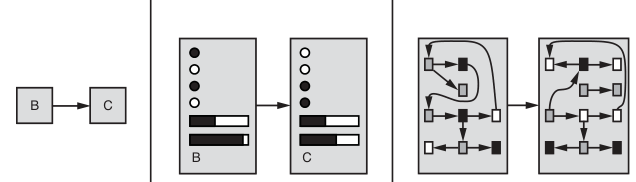
\includegraphics[width=\linewidth, height=2.5cm, keepaspectratio]{Pictures/ai-ml/agent-state-repr.png}
    \caption*{atomic, factored, and structured states}
\end{figure}

\begin{enumerate}
    \item \textbf{Atomic}
    \begin{enumerate}
        \item each state of the world is indivisible—it has no internal structure. 
    
        \item The algorithms underlying search and game-playing, Hidden Markov models, and Markov decision processes all work with atomic representations—or, at least, they treat representations as if they were atomic.

        \item if two different atomic states have nothing in common—they are just different black boxes
    \end{enumerate}

    \item \textbf{Factored}
    \begin{enumerate}
        \item A factored representation splits up each state into a fixed set of \textbf{variables} or \textbf{attributes}, each of which can have a \textbf{value}.

        \item two different factored states can share some attributes and not others; this makes it much easier to work out how to turn one state into another.

        \item With factored representations, we can also represent uncertainty\\
        \textbf{for example}, ignorance about the amount of gas in the tank can be represented by leaving that attribute blank.

        \item  Many important areas of AI are based on factored representations, including constraint satisfaction algorithms, propositional logic, planning, Bayesian networks, and the machine learning algorithms.
    \end{enumerate}

    \item \textbf{structured}
    \begin{enumerate}
        \item we need to understand the world as having things in it that are
related to each other, not just variables with values.

        \item Structured representations underlie relational databases and first-order logic, first-order probability models, knowledge-based learning and much of natural language understanding. 
        
        \item almost everything that humans express in natural language concerns objects and their relationships.
    \end{enumerate}

    \item  the axis along which atomic, factored, and structured representations lie is the axis of increasing \textbf{expressiveness}.\\
    a more expressive representation can capture, at least as concisely, everything a less expressive one can capture, plus some more.\\
    Often, the more expressive language is much more concise; for example, the rules of chess can be written in a page or two of a structured-representation language such as first-order logic but require thousands of pages when written in a factored-representation language such as propositional logic.\\
    On the other hand, reasoning and learning become more complex as the expressive power of the representation increases.\\
    To gain the benefits of expressive representations while avoiding their drawbacks, intelligent systems for the real world may need to operate at all points along the axis simultaneously.
\end{enumerate}

\section{Agent programs \cite{aci-1}}

\begin{enumerate}
    \item skeleton: they take the current percept as input from the sensors and return an action to the actuators. 
    
    \item agent program takes the current percept as input\\
    he agent program takes just the current percept as input because nothing more is available from the environment; if the agent’s actions need to depend on the entire percept sequence, the agent will have to remember the percepts.

    \item agent function takes the entire percept history
\end{enumerate}

\subsection{Table Driven Agent \cite{aci-1}}

\begin{algorithm}[H]
    \caption{The TABLE-DRIVEN-AGENT program is invoked for each new percept and returns an action each time. It retains the complete percept sequence in memory. \cite{aci-1}}

    \SetKwFunction{FUNCTION}{TABLE-DRIVEN-AGENT}
    \SetKwProg{Fn}{function}{:}{}
    \Fn{\FUNCTION{percept}}{
        \textbf{persistent}:\\
        \hspace{0.4cm} \textit{percepts}, a sequence, initially empty\\
        \hspace{0.4cm} \textit{table}, a table of actions, indexed by percept sequences, initially fully specified \\
        append \textit{percept} to the end of \textit{percepts} \\
        \textit{action} $\gets$ LOOKUP(\textit{percepts},\textit{table}) \\
        \Return \textit{action}
    }
\end{algorithm}

\vspace{0.3cm}

\begin{enumerate}
    \item If $\mathcal{P}$ be the set of possible percepts and let $\mathcal{T}$ be the lifetime of the agent (the total number of percepts it will receive), then The lookup table will contain $\dsum^T_{t=1} |P| ^t$ entries.

    \item Challenges if there are too many table entries:
    \begin{enumerate}
        \item storage space
        \item designer need time to create the table
        \item agent might never learn all the right table entries from its experience
        \item even if the environment is simple enough to yield a feasible table size, the designer still has no guidance about how to fill in the table entries
    \end{enumerate}

\end{enumerate}

\subsection{Simple reflex agents \cite{aci-1}}

\begin{table}[H]
    \begin{minipage}{0.4\linewidth}
        \begin{figure}[H]
            \centering
            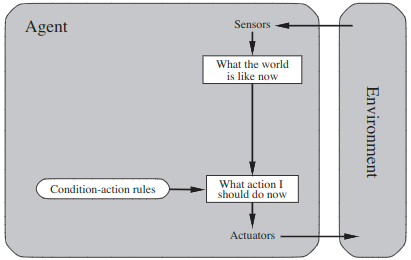
\includegraphics[width=\linewidth, height=4cm, keepaspectratio]{Pictures/ai-ml/agent--simple-reflex.png}
            \caption{Schematic diagram of a simple reflex agent}
        \end{figure}
    \end{minipage}
    \hfill
    \begin{minipage}{0.58\linewidth}
        \begin{algorithm}[H]
            \caption{simple reflex agent \cite{aci-1}}

            \SetKwFunction{FUNCTION}{SIMPLE-REFLEX-AGENT}
            \SetKwProg{Fn}{function}{:}{}
            \Fn{\FUNCTION{percept}}{
                \textbf{persistent}: \textit{rules}, a set of condition–action rules\\

                \textit{state} $\gets$ INTERPRET-INPUT(\textit{percept}) \\
                
                \textit{rule} $\gets$ RULE-MATCH(\textit{state,rules}) \\
                
                \textit{action} $\gets$ \textit{rule}.ACTION \\
                
                \textbf{return} \textit{action}
            }
        \end{algorithm}
    \end{minipage}
\end{table}

\vspace{0.3cm}

\begin{enumerate}
    \item The simplest kind of agent is the simple reflex agent. 
    
    \item These agents select actions on the basis of the current percept, ignoring the rest of the percept history.

    \item uses \textbf{condition–action rules} to map percepts to actions

    \item The \textbf{INTERPRET-INPUT function} generates an abstracted description of the current state from the percept, and the \textbf{RULE-MATCH function} returns the first rule in the set of rules that matches the given state description.

    \item Note that the description in terms of “rules” and “matching” is purely conceptual; actual implementations can be as simple as a collection of logic gates implementing a Boolean circuit.

\subsubsection*{DISADVANTAGES:}

    \item limited intelligence
    
    \item environment needs to be fully observable. Even a little bit of unobservability can cause serious trouble.
    
    \item Infinite loops are often unavoidable for simple reflex agents operating in partially observable environments\\
    \textbf{Solution}: Escape from infinite loops is possible if the agent can randomize its actions.\\
    In single-agent environments, randomization is usually not rational.\\
    It is a useful trick that helps a simple reflex agent in some situations, but in most cases we can do much better with more sophisticated deterministic agents. 
\end{enumerate}



\subsection{Model-based reflex agents \cite{aci-1}}

\begin{table}[H]
    \begin{minipage}{0.4\linewidth}
        \begin{figure}[H]
            \centering
            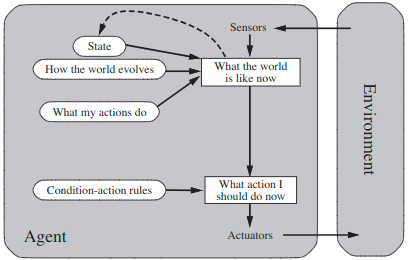
\includegraphics[width=\linewidth, height=4cm, keepaspectratio]{Pictures/ai-ml/agent--model-based-reflex.png}
            \caption{Model-based reflex agent}
        \end{figure}
    \end{minipage}
    \hfill
    \begin{minipage}{0.58\linewidth}
        \begin{algorithm}[H]
            \caption{model-based reflex agent \cite{aci-1}}

            \SetKwFunction{FUNCTION}{MODEL-BASED-REFLEX-AGENT}
            \SetKwProg{Fn}{function}{:}{}
            \Fn{\FUNCTION{percept}}{
                \textbf{persistent}:\\
                
                \hspace{0.4cm} \textit{state}, the agent’s current conception of the world state \\
                \hspace{0.4cm} \textit{model}, a description of how the next state depends on current state and action \\
                \hspace{0.4cm} \textit{rules}, a set of condition–action rules \\
                \hspace{0.4cm} \textit{action}, the most recent action, initially none \\

                \textit{state} $\gets$ UPDATE-STATE(\textit{state, action, percept, model}) \\
                
                \textit{rule} $\gets$ RULE-MATCH(\textit{state, rules}) \\
                
                \textit{action} $\gets$ \textit{rule}.ACTION \\
                
                \textbf{return} \textit{action}
            }
        \end{algorithm}
    \end{minipage}
\end{table}

\vspace{0.3cm}


\begin{enumerate}
    \item keeps track of the part of the world it can’t see now. (handle partial observability)\\
    The agent maintains some sort of \textbf{internal state} that depends on the percept history and thereby reflects at least some of the unobserved aspects of the current state.

    \item Updating this internal state information as time goes by requires two kinds of knowledge to be encoded in the agent program.
    \begin{enumerate}
        \item we need some information about how the world evolves independently of the agent

        \item we need some information about how the agent’s own actions affect the world
    \end{enumerate}
    This knowledge about “\textit{how the world works}” is called a \textbf{model} of the world. 

    \item The details of how models and states are represented vary widely depending on the type of environment and the particular technology used in the agent design. 

    \item Regardless of the kind of representation used, it is seldom possible for the agent to determine the current state of a partially observable environment exactly.\\
    Instead, the box\ mechanism labeled “what the world is like now” represents the agent’s “best guess” (or sometimes best guesses).
\end{enumerate}


\subsection{(Model-based) Goal-based agents \cite{aci-1}}

\begin{enumerate}
    \item as well as a current state description, the agent needs some sort of \textbf{goal} information that describes situations that are desirable

    \item \textbf{Search} and \textbf{planning} are the subfields of AI devoted to finding action sequences that achieve the agent’s goals.

    \item Although the goal-based agent appears less efficient, it is more flexible because the knowledge that supports its decisions is represented explicitly and can be modified.\\
    If it starts to rain, the agent can update its knowledge of how effectively its brakes will operate; this will automatically cause all of the relevant behaviors to be altered to suit the new conditions.\\
    For the reflex agent, on the other hand, we would have to rewrite many condition–action rules. 

    \item Goals alone are not enough to generate high-quality behavior in most environments.
\end{enumerate}


\begin{table}[h]
    \begin{minipage}{0.49\linewidth}
        \begin{figure}[H]
            \centering
            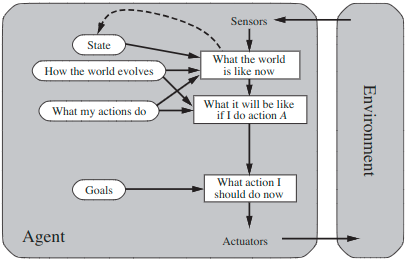
\includegraphics[width=\linewidth, height=4cm, keepaspectratio]{Pictures/ai-ml/agent--model-based-goal-based.png}
            \caption{Model-based goal-based agent \cite{aci-1}}
        \end{figure}
    \end{minipage}
    \hfill
    \begin{minipage}{0.49\linewidth}
        \begin{figure}[H]
            \centering
            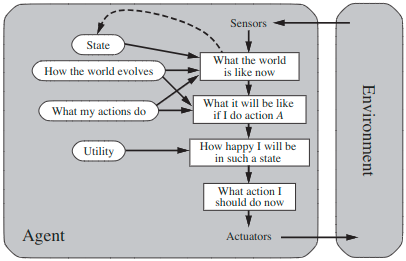
\includegraphics[width=\linewidth, height=4cm, keepaspectratio]{Pictures/ai-ml/agent--model-based-utility-based.png}
            \caption{Model-based utility-based agent \cite{aci-1}}
        \end{figure}
    \end{minipage}
\end{table}

\subsection{Utility-based agents \cite{aci-1}}

\begin{enumerate}
    \item Many action sequences can lead to same goal, but some sequences are more favourable than others.\\
    Goals just provide a crude binary distinction between “happy” and “unhappy” states.\\
    A more general performance measure should allow a comparison of different world states according to exactly how happy they would make the agent.\\
    Because “happy” does not sound very scientific, economists and computer scientists use the term \textbf{utility} instead.

    \item An agent’s \textbf{utility function} is essentially an internalization of the performance measure. 
    
    \item If the internal utility function and the external performance measure are in agreement, then an agent that chooses actions to maximize its utility will be rational according to the external performance measure. 

    \item like goal-based agents, a utility-based agent has many advantages in terms of flexibility and learning.

    \item in two kinds of cases, goals are inadequate but a utility-based agent can still make rational decisions. 
    \begin{enumerate}
        \item when there are conflicting goals, only some of which can be achieved (for example, speed and safety), the utility function specifies the appropriate tradeoff.

        \item when there are several goals that the agent can aim for, none of which can be achieved with certainty, utility provides a way in which the likelihood of success can be weighed against the importance of the goals. 
    \end{enumerate}

    \item An agent that possesses an \textbf{\textit{explicit} utility function} can make rational decisions with a general-purpose algorithm that does not depend on the specific utility function being maximized.\\
    In this way, the “global” definition of rationality—designating as rational those agent functions that have the highest performance—is turned into a “local” constraint on rational-agent designs that can be expressed in a simple program.

    \item A utility-based agent has to model and keep track of its environment, tasks that have involved a great deal of research on perception, representation, reasoning, and learning. \\
    Choosing the utility-maximizing course of action is also a difficult task, requiring ingenious algorithms.
\end{enumerate}


\subsection{Learning Agent \cite{aci-1}}

\begin{figure}[H]
    \centering
    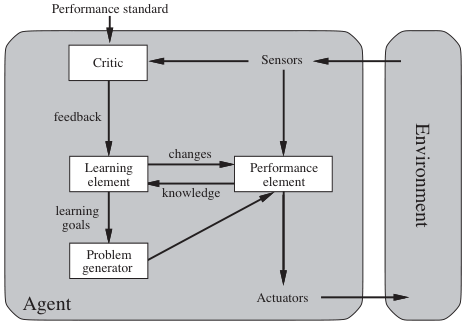
\includegraphics[width=\linewidth, height=4cm, keepaspectratio]{Pictures/ai-ml/agent--learning.png}
    \caption{General Learning Agent \cite{aci-1}}
\end{figure}


\begin{enumerate}
    \item Learning allows the agent to operate in initially unknown environments and to become more competent than its initial knowledge alone might allow.

    \item A learning agent can be divided into four conceptual components:
    \begin{enumerate}
        \item \textbf{learning element}: responsible for making improvements

        \item \textbf{performance element}: responsible for selecting external actions\\
        it takes in percepts and decides on actions

        \item \textbf{critic}: provides feedback on how the agent is doing and determines how the performance element should be modified to do better in the future\\
        The critic tells the learning element how well the agent is doing with respect to a fixed performance standard.\\
        The critic is necessary because the percepts themselves provide no indication of the agent’s success.

        \item \textbf{problem generator}: It is responsible for suggesting actions that will lead to new and informative experiences.\\
        The point is that if the performance element had its way, it would keep doing the actions that are best, given what it knows.\\
        But if the agent is willing to explore a little and do some perhaps sub-optimal actions in the short run, it might discover much better actions for the long run.\\
        The problem generator’s job is to suggest these exploratory actions.
    \end{enumerate}

    \item  the \textbf{performance standard} distinguishes part of the
incoming percept as a reward (or penalty) that provides direct feedback on the quality of the
agent’s behavior.    
\end{enumerate}



\subsection{problem-solving agent \cite{aci-1}}

\begin{enumerate}
    \item Problem-solving agents use \textbf{atomic} representations, states of the world are considered as wholes, with no internal structure visible to the problem-solving algorithms. 

    \item \textbf{uninformed search algorithms}—algorithms that are given no information about the problem other than its definition.

    \item \textbf{Informed search algorithms} can do quite well given some guidance on where to look for solutions

    \item \textbf{Goals} help organize behavior by limiting the objectives that the agent is trying to achieve and hence the actions it needs to consider.\\
    \textbf{Goal formulation}, based on the current situation and the agent’s performance measure, is the first step in problem solving.\\
    We consider a goal to be a set of world states—exactly those states in which the goal is satisfied.\\
    The agent’s task is to find out how to act, now and in the future, so that it reaches a goal state.

    \item  \textbf{Problem formulation} is the process of deciding what actions and states to consider, given a goal. 

    \item The process of looking for a sequence of actions that reaches the goal is called \textbf{search}.

    \item A search algorithm takes a problem as input and returns a \textbf{solution} in the form of an \textbf{action sequence}.\\
    Solution quality is measured by the path cost function, and an \textbf{optimal solution} has the lowest path cost among all solutions.

    \item Once a solution is found, the actions it recommends can be carried out. This is called the \textbf{execution phase}.

    \item A \textbf{problem} can be defined formally by five components:
    \begin{enumerate}
        \item The \textbf{initial state} that the agent starts in.

        \item A description of the possible \textbf{actions} available to the agent.\\
        Given a particular state \textit{s}, \verb|ACTIONS(s)| returns the set of actions that can be executed in \textit{s}.\\
        We say that each of these actions is \textbf{applicable} in \textit{s}.

        \item A description of what each action does; the formal name for this is the \textbf{transition model}, specified by a function \verb|RESULT(s, a)| that returns the state that results from doing action \textit{a} in state \textit{s}.\\
        We also use the term \textbf{successor} to refer to any state reachable from a given state by a single action.\\
        Together, the initial state, actions, and transition model implicitly define the \textbf{state space} of the problem—the set of all states reachable from the initial state by any sequence of actions.\\
        The state space forms a directed network or graph in which the nodes are states and the links between nodes are actions.\\
         A \textbf{path} in the state space is a sequence of states connected by a sequence of actions.

        \item \textbf{goal test} determines whether a given state is a goal state.

        \item The \textbf{step cost} of taking action $a$ in state $s$ to reach state $s'$ is denoted by $c(s, a, s')$.\\
        A \textbf{path cost} function that assigns a numeric cost to each path.\\
        The problem-solving agent chooses a cost function that reflects its own performance measure.\\
        we assume that the cost of a path can be described as the \textbf{sum} of the costs of the individual actions along the path.
    \end{enumerate}

    \item A \textbf{toy problem}\indexlabel{toy problem} is intended to illustrate or exercise various problem-solving methods.\\
    It can be given a concise, exact description and hence is usable by different researchers to compare the performance of algorithms.

    \item A \textbf{real-world problem}\indexlabel{real-world problem} is one whose solutions people actually care about.\\
    Such problems tend not to have a single agreed-upon description, but we can give the general flavor of their formulations.
\end{enumerate}

\begin{figure}[H]
    \centering
    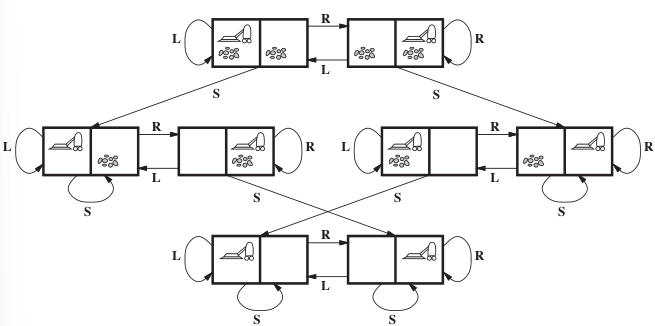
\includegraphics[width=\linewidth, height=6cm, keepaspectratio]{Pictures/ai-ml/vaccum-toy-states.png}
    \caption*{The state space for the vacuum world. Links denote actions: L = Left, R = Right, S = Suck.}
\end{figure}

\begin{customTableWrapper}{1.3}
\begin{longtable}{|p{3cm} p{10cm}|}
    \hline\endfirsthead
    \hline\endhead
    \hline\endfoot
    \hline\endlastfoot

    \textbf{States} & The state is determined by both the agent location and the dirt locations. \\ 
    \hline

    \textbf{Initial state} & Any state can be designated as the initial state.\\
    \hline

    \textbf{Actions} & In this simple environment, each state has just three actions: Left, Right, and Suck.\\
    \hline

    \textbf{Transition model} & The actions have their expected effects, except that moving Left in the leftmost square, moving Right in the rightmost square, and Sucking in a clean square have no effect. \\
    \hline

    \textbf{Goal test} & This checks whether all the squares are clean.\\
    \hline

    \textbf{Path cost} & Each step costs 1, so the path cost is the number of steps in the path.\\
    \hline
\end{longtable}
\end{customTableWrapper}

\begin{algorithm}[h]
    \caption*{A simple problem-solving agent. It first formulates a goal and a problem, searches for a sequence of actions that would solve the problem, and then executes the actions one at a time. When this is complete, it formulates another goal and starts over. \cite{aci-1}}

    \SetKwFunction{FUNCTION}{SIMPLE-PROBLEM-SOLVING-AGENT}
    \SetKwProg{Fn}{function}{:}{}
    \Fn{\FUNCTION{percept}}{
        \textbf{persistent}:\\
        \hspace{0.4cm} \textit{seq}, an action sequence, initially empty \\
        \hspace{0.4cm} \textit{state}, some description of the current world state \\
        \hspace{0.4cm} \textit{goal}, a goal, initially null \\
        \hspace{0.4cm} \textit{problem}, a problem formulation\\
        
        state $\gets$ UPDATE-STATE(\textit{state, percept})\\
        \If{\textit{seq} is empty}{
            \textit{goal} $\gets$ FORMULATE-GOAL(\textit{state})\\
            
            \textit{problem} $\gets$ FORMULATE-PROBLEM(\textit{state, goal})\\
            
            \textit{seq} $\gets$ SEARCH(\textit{problem})\\
            
            \If{\textit{seq} = \textit{failure}}{
                \textbf{return} a null action
            }
        }
        \textit{action} $\gets$ FIRST(\textit{seq})\\
        \textit{seq} $\gets$ REST(\textit{seq})\\
        \textbf{return} \textit{action}
    }
\end{algorithm}


\subsubsection{Measuring problem-solving performance \cite{aci-1}}

\begin{customTableWrapper}{1.2}
\begin{table}[H]
    \centering
    \begin{tabular}{l p{10cm}}
        \textbf{Completeness} & Is the algorithm guaranteed to find a solution when there is one? \\
        
        \textbf{Optimality} & Does the strategy find the optimal solution? \\
        
        \textbf{Time complexity} & How long does it take to find a solution? \\
        
        \textbf{Space complexity} & How much memory is needed to perform the search?\\
    \end{tabular}
\end{table}
\end{customTableWrapper}


\begin{customTableWrapper}{1.2}
\begin{table}[H]
    \centering
    \begin{tabular}{l p{10cm}}
        $V$ & set of vertices (nodes) of the graph \\
        
        $E$ & set of edges (links) \\

        $b$ & \textbf{branching factor} or maximum number of successors of any node\\

        $d$ & \textbf{depth} of the shallowest goal node (i.e., the number of steps along the path from the root)\\

        $m$ &  maximum length of any path in the state space\\
    \end{tabular}
    \caption*{Notation}
\end{table}
\end{customTableWrapper}



\begin{enumerate}
    \item Time and space complexity are always considered with respect to some measure of the problem difficulty. 
    
    \item In theoretical computer science, the typical measure is the size of the state space graph, $|V| + |E|$.

    \item \textbf{search cost}: typically depends on the time complexity but can also include a term for memory usage

    \item \textbf{total cost}: combines the search cost and the path cost of the solution found
\end{enumerate}





\subsection{planning agents \cite{aci-1}}

\begin{enumerate}
    \item Goal-based agents that use more advanced \textbf{factored} or \textbf{structured} representations are usually called \textbf{planning agents}.


\end{enumerate}





% 79/1153

































































